\documentclass[conference]{IEEEtran}
\IEEEoverridecommandlockouts
% The preceding line is only needed to identify funding in the first footnote. If that is unneeded, please comment it out.
\usepackage{cite}
\usepackage{amsmath,amssymb,amsfonts}
\usepackage{algorithmic}
\usepackage{graphicx}
\usepackage{textcomp}
\usepackage{xcolor}
\usepackage{url}
\usepackage{tabularx}
\usepackage{tabulary}
\usepackage{svg}
\usepackage[scaled=0.8]{FiraMono}

\def\BibTeX{{\rm B\kern-.05em{\sc i\kern-.025em b}\kern-.08em
    T\kern-.1667em\lower.7ex\hbox{E}\kern-.125emX}}
\begin{document}

\title{\textsc{Ferret Miner}: A Process Mining Case Study}

\author{\IEEEauthorblockN{Martin Alvarez-Lopez${}^1$\thanks{${}^1$ MS Candidate in Software Engineering, San José State University}}
% \IEEEauthorblockA{San José State University}
\and
\IEEEauthorblockN{Carlos Hernandez${}^2$\thanks{${}^2$ MS Candidate in Computer Engineering, San José State University}}
% \IEEEauthorblockA{San José State University}
\and
\IEEEauthorblockN{Hardy Leung${}^3$\thanks{${}^3$ MS Candidate in Artificial Intelligence, San José State University}}
% \IEEEauthorblockA{San José State University}
\and
\IEEEauthorblockN{Divyam Sobti${}^3$}
% \IEEEauthorblockA{San José State University}
}

\maketitle

\begin{abstract}
The objective of this project is to analyze event data logs from
the travel reimbursement process at Eindhoven University of Technology
(ETU/c), identify bottlenecks in the process, and
seek improvement to its efficiency.
We process and filter the event data, and then generate simplified and
representative process models to help locate where
the most time-consuming and impactful critical tasks are.
Our analysis suggests that
improvement in the supervisor appproval and payment handling activities 
could significantly
reduce the time processing the travel reimbursement.
\end{abstract}

\begin{IEEEkeywords}
process mining, data mining, conformance, event logs, business intelligence
\end{IEEEkeywords}

\section{Introduction}
\label{section-intro}


Nowadays, most organizations use information systems to support
the execution of their business processes, generating significant
amounts of data.
Mainstream information systems, such as Enterprise Resource
Planning (ERP), Work on Management Systems (WMS), and Customer
Relationship Management (CRM), have become vital tools behind the
operation of almost 
any company process\cite{Tuto2022}. All of these platforms
offer rich event logging capabilities, in which
an event log is
basically a record of an activity performed with a timestamp embedded
\cite{Proc2022}.

As a result, there are plenty of oppportunities, through
proper supervision of business behavior, to identify and adjust
tasks that are generating problems for the business processes
\cite{LeAl1994}.
One important technique to accomplish such goal is process mining, a
specialized data analysis technique that reveal core business behavior
indicated by activity logs.
Process mining would start with these event logs, extracting important
information including the chronology of the activities
 and their execution time registered in each log. Representative models
would be built, or discovered automatically,
and then be used to detect errors and deficiencies in the process,
and to provide insight and suggestions for process enhancement.
Process mining is most closely related to data mining 
amongst business intelligence disciplines. However,
data mining concentrates on finding relationships among data,
whereas process mining also looks at data from a systematic
perspective.

\subsection{Problem Description}

This project is a process mining case study designed to
identify patterns,
delays and bottlenecks that obstruct the efficient flow of the process
activities. Specifically, we studied a dataset with
real-life event log data from the travel reimbursement process at
Eindhoven University of Technology (ETU/e).
The event logs provide a detailed record of the travel reimbursement process,
including important attributes such as identification, resource,
timestamp, permits, payment and budgetting information, and event labels.
Students or staff would submit their reimbursement application,
provide suppport documentation (if traveling internationally), wait for
reimbursement decision and subsequent payment, and possibly deal with
rejection and resubmission. All of these information is captured in the
event log.
Collectively, these information provided a substantial amount of detail
into the process. 
The data was obtained from 
the annual Business Process Intelligence Challenge (BPI Challenge)
as part of
the 2020 International Conference on Process Mining held in Padova, Italy
\cite{BPI2020}, and has been
pre-processed and anonymized for research purpose.

Our approach to process mining is based on the work by
Wil Van Der Aalst in his seminal paper titled simply
``Process Mining,'' \cite{van2012},
where process mining guidelines are detailed.
A process mining implementation generally
covers three main issues: (1) discovery, (2) conformance,
and (3) enhancement.
Our project focuses on discovery since it is the area
that requires more effort and it is the most deterministic for the
success of the analysis. That said, we shall also take a cursory
look at conformance analysis as an aide to discovery,
 and to motivate our future work.

\subsection{Motivation}

Publications on practical application of process mining are scarce,
and our research paper aims to add support to this section. Our goal is
to demonstrate the practicality of process mining analysis
in practice, in application to the real-life travel reimbursement problem
as detailed earlier.

Furthermore, we are very interested in the evaluation and application
of a relatively new process mining technique based on
the Python-based process mining library called \textsc{pm4py}
developed by Berti, van Zelst, and van der Aalst \cite{BeZe2019}.
According to the authors,
\textsc{pm4py} is a modern, open-source, and emerging platform developed
specifically for the data science community. Prior to the turn of the
millenium,
there were hardly any tooling for process mining, but
since then a slew of software tools, both open-source
(ProM and Apromore) and commercial (Disco, Celonis, and ProcessGold),
have been developed. Yet, many were proprietary, hard to extend,
hiding behind graphical user interfaces, or (worst yet) all of the above.
The mindset of process mining
tooling contrasted greatly with the modern philosophy of data science R\&D,
which put significant emphasis on openness and extensibility.
\textsc{pm4py} was developed to bridge the gap
between old-style process mining and modern data science
capabilities including
\texttt{Pandas}, \texttt{NumPy}, \texttt{scikit-learn}.

We whole-heartedly
agree with the assessment of the authors, and we look further at opportunities
that the \textsc{pm4py} approach brought forward, including the
the adoption of modern and rapidly evolving machine learning
functionalities to process mining.


\subsection{Approach Summary}

The document is structured as follows: Section \ref{section-intro} provides details about
process mining and its fundamentals; Section \ref{section-survey} presents an overview of
our approach and related literature review; Sections \ref{section-technical}
and \ref{section-methodology} analyzes the
outcomes produced from our primary studies and research problem,
and section \ref{section-models} focuses on the process models we built
and the analysis that follows. Section \ref{section-future}
refers to our discussion about future work. We will conclude our paper
in \ref{section-conclusion}.

\section{Survey}
\label{section-survey}

In this section, we shall offer a very brief review of the literature
on process mining, focusing on the development of techniques
and algorithms from a control-flow discovery perspective, as well as
 its applications.

\subsection{Process Mining}

Van der Aalst et al.~described the discipline of process mining as positioned
somewhere between data mining and process modeling
\cite{van2004}. Process mining interacts with the rest of the software
ecosystem
mainly through the language of event logs (see Figure \ref{fig-outline}),
and the objective is to provides useful information
with implication on the business processes, organizations, and people involved.

\begin{figure}[htbp]
\centerline{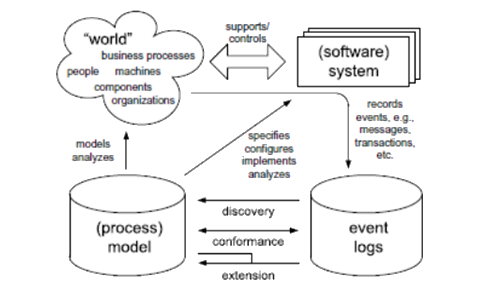
\includegraphics[width=0.4\textwidth]{images/image2a.png}}
\caption{General outline of process mining approach.}
\label{fig-outline}
\end{figure}

Although information system databases capture important business data
in the form of event logs, these systems do not
usually provide understanding of the data in a structural or systematic manner.
Traditionally, process analysts must search for and
retrieve the information directly from the system, and perform manual
analysis to accomplish their specific objectives.
Another way to put it is that event logs only possess
the right information, but not necessarily the right insight, to determine the
behavior of the system.
Whether or not a process mining implementation is successful or
applicable thus largely hinges on what it can do with the event logs
\cite{van2012}. As such, process mining approach must
embrace three main actions (Figure \ref{fig-layout}):

\begin{itemize}
\item \textit{Discovery} --
to create robust and representative process models through
 analyzing event logs.

\item \textit{Conformance} -- to verify and compare newly created
models against either the event logs or other predefined models
to gain knowledge.

\item \textit{Enhancement} -- to turn the analysis 
models into insights and suggestions to overcome previously
detected problems.
\end{itemize}

\begin{figure}[htbp]
\centerline{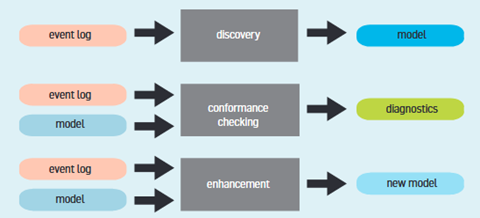
\includegraphics[width=0.5\textwidth]{images/image1.png}}
\caption{General outline of process mining approach.}
\label{fig-layout}
\end{figure}

\subsection{Process Models}

Many distinct data analysis approaches have been developed to discover
processes from event logs. However, Petri nets\footnote{and the
equivalent BPMN models and process trees} have become a
widely adopted technique over other approaches \cite{Cook1998} due to their
intuitiveness, mathematical soundness, and ease of analysis.
Another approach utilizes Unified
Modeling Language (UML) diagrams \cite{Sait2019}.
In 2004, Van der Wilst et al.~described the 
a novel algorithm
called \textsc{alpha miner}\cite{van2004} which
is capable of depicting event data logs into
work-flow diagrams, which can be translated to Petri nets.
The success of \textsc{alpha miner} has inspired many follow-up publications,
including a popular model
called \textsc{flexible heuristic miner} \cite{Weij2006}.
One main characteristic of this
algorithm is to be highly permissive in controling statistical levels and
threshold adjustment. In order to deal with the
massive number of events that actual information systems generate,
Burattin et al. \cite{Bura2014} developed another extension to
\textsc{heuristic miner} based on
lossy counting, as well as a sliding window that effectively analyzes
streams of real datasets.

\subsection{Applications}

Most process mining publications are dedicated mainly to the enhancement
of novel methodologies and algorithms with significant emphasis on the
control-flow discovery area \cite{van2004}. However, the public services area
has been fruitful ground
for process mining development research. For instance, a
Genetic Miner approach was tested by Alves de Madeiros et al. \cite{deMe2007}
in Dutch municipalities. Additionally, van del Aalst et al. \cite{RoDJ2009}
applied an analysis of organizations in another municipality process.
Rozinat et al. \cite{RoMa2009} evaluated process models in two different case
studies on the public sector.

Nonetheless, all these research
applications are focused to validate and assess rather than enhance the
process. Implementation of process mining approaches have been also
developed in the private domain. Distinct discovery approaches were
deployed by Goedertier et al. \cite{GoDW2011} in the telecom field. Also, Mans
et al. \cite{MaSc2008} and Rebuge and Ferreira \cite{ReBu2012} created a convoluted
process mining method to resolve the tracking of patients within the
healthcare industry.

The literature mentioned above provides the fundamentals of process mining from a general perspective. Each approach contributes significantly to the process mining study field, and in this paper, we focus on its application. 

\section{Technical Approach}
\label{section-technical}

We shall briefly describe our approach to answering the questions of
where the bottlenecks are. We would first properly clean the event logs,
and then build a model that best captures the behavior of the
process (in other words, to mine the process), making the proper tradeoff
between robustness, accuracy, and coverage.  Then, we will use the
chosen model to answer the questions we have in mind.

We shall note that process mining is a relatively new techniques, and
as such we spent a disproportional amount of time ramping up the project.
While \textsc{pm4py}, in essence an academic software,
was a great choice compared to other proprietary enterprise software
due to its focus on discovery algorithms and availability on Python,
it was nonetheless relatively immature and early in its development, and
hence suffered from instability. The visualization capability was clearly
inadequate, and it offered very little flexibility as far as exploration
is concerned.

\section{Methodology}
\label{section-methodology}

In this section we will discuss about data, how we preprocessed the data, which model we used, how we reach the result and disscuss about the result.

\subsection{Description of the Dataset}

After clear understanding of the question we got to know that we had to
 find bottleneck in travel declaration.
After reviewing the data provided to us we  decided to go with the domestic
and internation declaration.
Both the dataset are in XES format,
an XML-based standard for event logs \cite{XES2021}.
It contains the information regarding the process that is
they contains event log. The events are organized in a two-level hierarchy --
the log is made of a collection of cases (also known as traces in technical
term), and each case is made of a collection of events. Both cases and
events are extensible constructs to allow for maximum flexibility in
modeling events for different needs.



As we imported the logs into Python via \textsc{pm4py}, in their simplest form the
log is organized into a Python dataframe, a key construct of
\texttt{Pandas}, the popular Python Data Analysis Library. However, as
dataframes are not hierarchical, \textsc{pm4py} flattene the log such that the
cases, and case attributes, become attributes of events. Therefore, if
there are $A_c$ case attributes in the case, and $A_e$ event attributes in the
XML specification, after \textsc{pm4py} import, we obtain a dataframe 
with $N$ observations, a total of $A_c + A_e$ attributes.

In our project,
the domestic process log is organized differently than
the international process log.  For domestic trip, an employee would first
complete the trip and then ask for reimbursement. On the other hand,
the policy for international trips mandates that
employees first obtain travel permits from the supervisor prior to
commencing the trips.

As a result, we are dealing with a more complex process in the case of
international travel, and the formal specification that describes
international cases also contain more fields.
Specifically, domestic cases have 5 attributes
each, and international cases have additional 13 attributes, together
with the 5 attributes shared with domestic cases
(\texttt{id}, \texttt{concept:name}, \texttt{BudgetNumber},
\texttt{DeclarationNumber}, \texttt{Amount}), for a total of 18 attributes.
In either case,
the raw event in the XES hierarchy has the same 5 attributes
(\texttt{id}, \texttt{org:resource}, \texttt{concept:name},
\texttt{time:timestamp}, and \texttt{org:role}).
After flattening, we
have the domestic dataframe with $56437$ events and $5+5=10$ attributes, and
the international dataframe with $72151$ events and $18+5=23$ attributes.
To avoid namespace collision, all case attributes were prefixed with
\texttt{case:} by \textsc{pm4py} (for example, the \texttt{id} field of a case
became \texttt{case:id} after flattening). Please refer to Tables
\ref{table-event}, 
\ref{table-domestic}, and
\ref{table-international} for a complete list of attributes:

\begin{table}[htbp]
\caption{XES Event Attributes (5 Total)}
% \vspace{-1em}
\begin{center}
\begin{verbatim}
    ---------------------------------------------------------
    id, org:resource, concept:name, time:timestamp, org:role
    ---------------------------------------------------------
\end{verbatim}
\end{center}
\label{table-event}
\end{table}

% \vspace{-1em}
\begin{table}[htbp]
\caption{XES Domestic Case Attributes (5 Total)}
% \vspace{-1em}
\begin{center}
\begin{verbatim}
    ---------------------------------------------------------
    id, concept:name, BudgetNumber, DeclarationNumber, Amount
    ---------------------------------------------------------
\end{verbatim}
\end{center}
\label{table-domestic}
\end{table}

% \vspace{-1em}
\begin{table}[htbp]
\caption{XES International Cases (18 fields)}
% \vspace{-1em}
\begin{center}
\begin{verbatim}
    ---------------------------------------------------------
    Permit travel permit number, DeclarationNumber, Amount,
    RequestedAmount, Permit TaskNumber, Permit BudgetNumber,
    OriginalAmount, Permit ProjectNumber, concept:name,
    Permit OrganizationalEntity, travel permit number,
    Permit RequestedBudget, id, Permit ID, Permit id,
    BudgetNumber, Permit ActivityNumber, AdjustedAmount        
    ---------------------------------------------------------
\end{verbatim}
\end{center}
\label{table-international}
\end{table}

\subsection{Data Preprocessing I -- Missing Values}

% Unique noise coming from outside processes, difficult to identify.
% Cannot use statistics to view outliers. There were no null or missing values.

Prior to process mining, we performed a thorough evaluation of the
domestic and international dataframes to ensure the best possible starting
point for analysis. There were three categories of modification we applied
to the datasets:

While we did not find any missing value per se (as far
as what \texttt{Pandas} is concerned), we did find columns with values of
the form ``\texttt{UNKNOWN}'' or ``\texttt{MISSING}'' as string. We
carefully evaluated what to do with these attributes on a case-by-case
basis. For example, we could drop the column (attribute), drop the row
(event), fill the missing values, or simply ignore the column.

In the case of international reimbursement, we decided that we should
drop events without a permit number. The permit number is actually a
concept of the case, and hence we were removing traces without permit
number in their entirety. This would turn out to be the most significant
modification to our international dataset.
% , reducing the number of events
% from 72151 to 45045, or 38\%.
We believe this is justified, because a trip
without any associated permit violated the very fundamental assumption
about the international reimbursement process, that there is a permit
associated with the trip. Note that the decision to drop these entries was
not ``lossy'', because international reimbursement request without a permit
number \underline{should} have been rejected and not entered into the system
in the first place.

\subsection{Data Preprocessing II -- Duplicated Attributes}

Perhaps due to prior inconsistency between
versions of the enterprise software, there are fields that are similar
or duplicate of each other. For example, \texttt{Permit ID}, \text{Permit id},
and \texttt{Permit travel permit number} may refer to the same thing.
Moreover, it is more than likely that exactly one of the three fields were
filled, while the other two had missing values (or reported as
``\texttt{MISSING}''. We combined these similar fields into one, picking out
the value from the non-missing column, and dropped the duplicates. Note that 
we performed this duplicate analysis prior to future treatment of missing
values.

As a result of these cleaning procedures, the size of the
the international dataframe was reduced from 72151 to 43707 (a 60\% drop),
with the
missing permit accounting for 95\% of such reduction. The number of
columns was reduced from 23 to 19, having dropped
several permit-related columns that are duplicates.

The domestic dataframe was also modified to a much small extent. The
number of events was reduced from 55087, a mere 2\% drop.

\subsection{Data Preprocessing III -- Infrequent Events}

Process models that can explain all possible event traces could be
arbitrarily complex. For example, obviously we would expect reimbursement to
be paid out only after the request was approved. But what if there is
a trace with a missing approval due to erroneous logging? A process model
built to handle 100\% of traces must then be able to handle a flow with
payment before request. Not only would the model be complex and clumsy,
it would also fail our objective.

A naive approach is to remove events that are uncommon, but doing so may
not be sufficient. For example, using the previous example,
while \textsc{request approved} that happened after \textsc{payment handled}
might be a rare sequence, neither of these events were rare.

In \textsc{pm4py} terminology, the variants of an event log is the
union of all possible sequences of event execution. For example, there are
68 variants in the domestic log, and 464 variants in the international log.
In fact, the above example
points to the need to remove traces that are uncommon. Clearly, it could
be beneficial to have the choice to build the process model based on
only the most popular traces. In fact, this was an important part of our
methodology and we shall take a closer look in the next section.

\section{Models and Results}
\label{section-models}


With the event logs new well understood and properly prepared, we are now
ready to consider building the actual process model.

\subsection{Choice of Models}

We must first answer the
question of what formal model to use. Our choices include BPMN\footnote{BPMN stands for Business Process Model Notation}  model,
process tree, Petri net, and Directly-Follows Graph (DFG). The
first three are mathematically equivalent and inter-changeable. On the other
hand, DFG shows a different view of BPMN graph constructed by aggregrating all possible link
between any pair of events that follows each other.

There are pros and cons in choosing Petri net vs DFG. DFGs can be constructed
directly from the event logs, and are simple to understand. Petri nets (as well
as the equivalents) can only be generated heuristically, for example, 
through inductive or heuristics miners (which \textsc{pm4py} supports).
The difference mainly lies on how concurrency is handled. For example,
say there are two activities $X$ and $Y$ that are sandwiched between
$A$ and $B$. In other words, the following are both legitimate sequence
of executions:

$\phantom{xxxxx}A \rightarrow X \rightarrow Y \rightarrow B$

$\phantom{xxxxx}A \rightarrow Y \rightarrow X \rightarrow B$


While both Alpha Miner and Inductive Miner would correctly deduct
(probabilistically) that $X$ and $Y$ have no inter-dependency but are
instead concurrent events, DFG would not be able to discern that, because
all it saw was $Y$ directly follows $X$ in the first example, and
$X$ directly follows $Y$ in the second. As a result, concurrency would
show up in DFGs as tight loops between two activities, yet there is no
way to prove that tight loops imply concurrency. As a result, if DFGs
become too complicated, they will confuse rather than aide reasoning.

For our purpose, however, we still believe 
is the preferred approach as the statistics on the edges of a DFG can be
made readily available, and more easily reasoned with. We just need to make
sure we have a model that is not too complicated.

How many top variants do we use to build the model?
We did experiment with different values of $k$, where $k$ is the number of
top variants (of the cleaned dataframe) to be used to build the DFG. We
evaluated many factors, though somewhat informally, and came to the conclusion
that we got the best balance between coverage and robustness if
we keep approximately 15 to 25\% of the top variants, depending on data
(higher for domestic, and lower for international). Figures~\ref{fig-domestic}
and \ref{fig-international} shows the DFG models we picked for
domestic and international reimbursement respectively. In each figure,
the DFG to the left is annotated with the number of directly following
edges, and the DFG to the right is annotated with the mean duration between
the two events.

\begin{figure*}[htbp]
\centerline{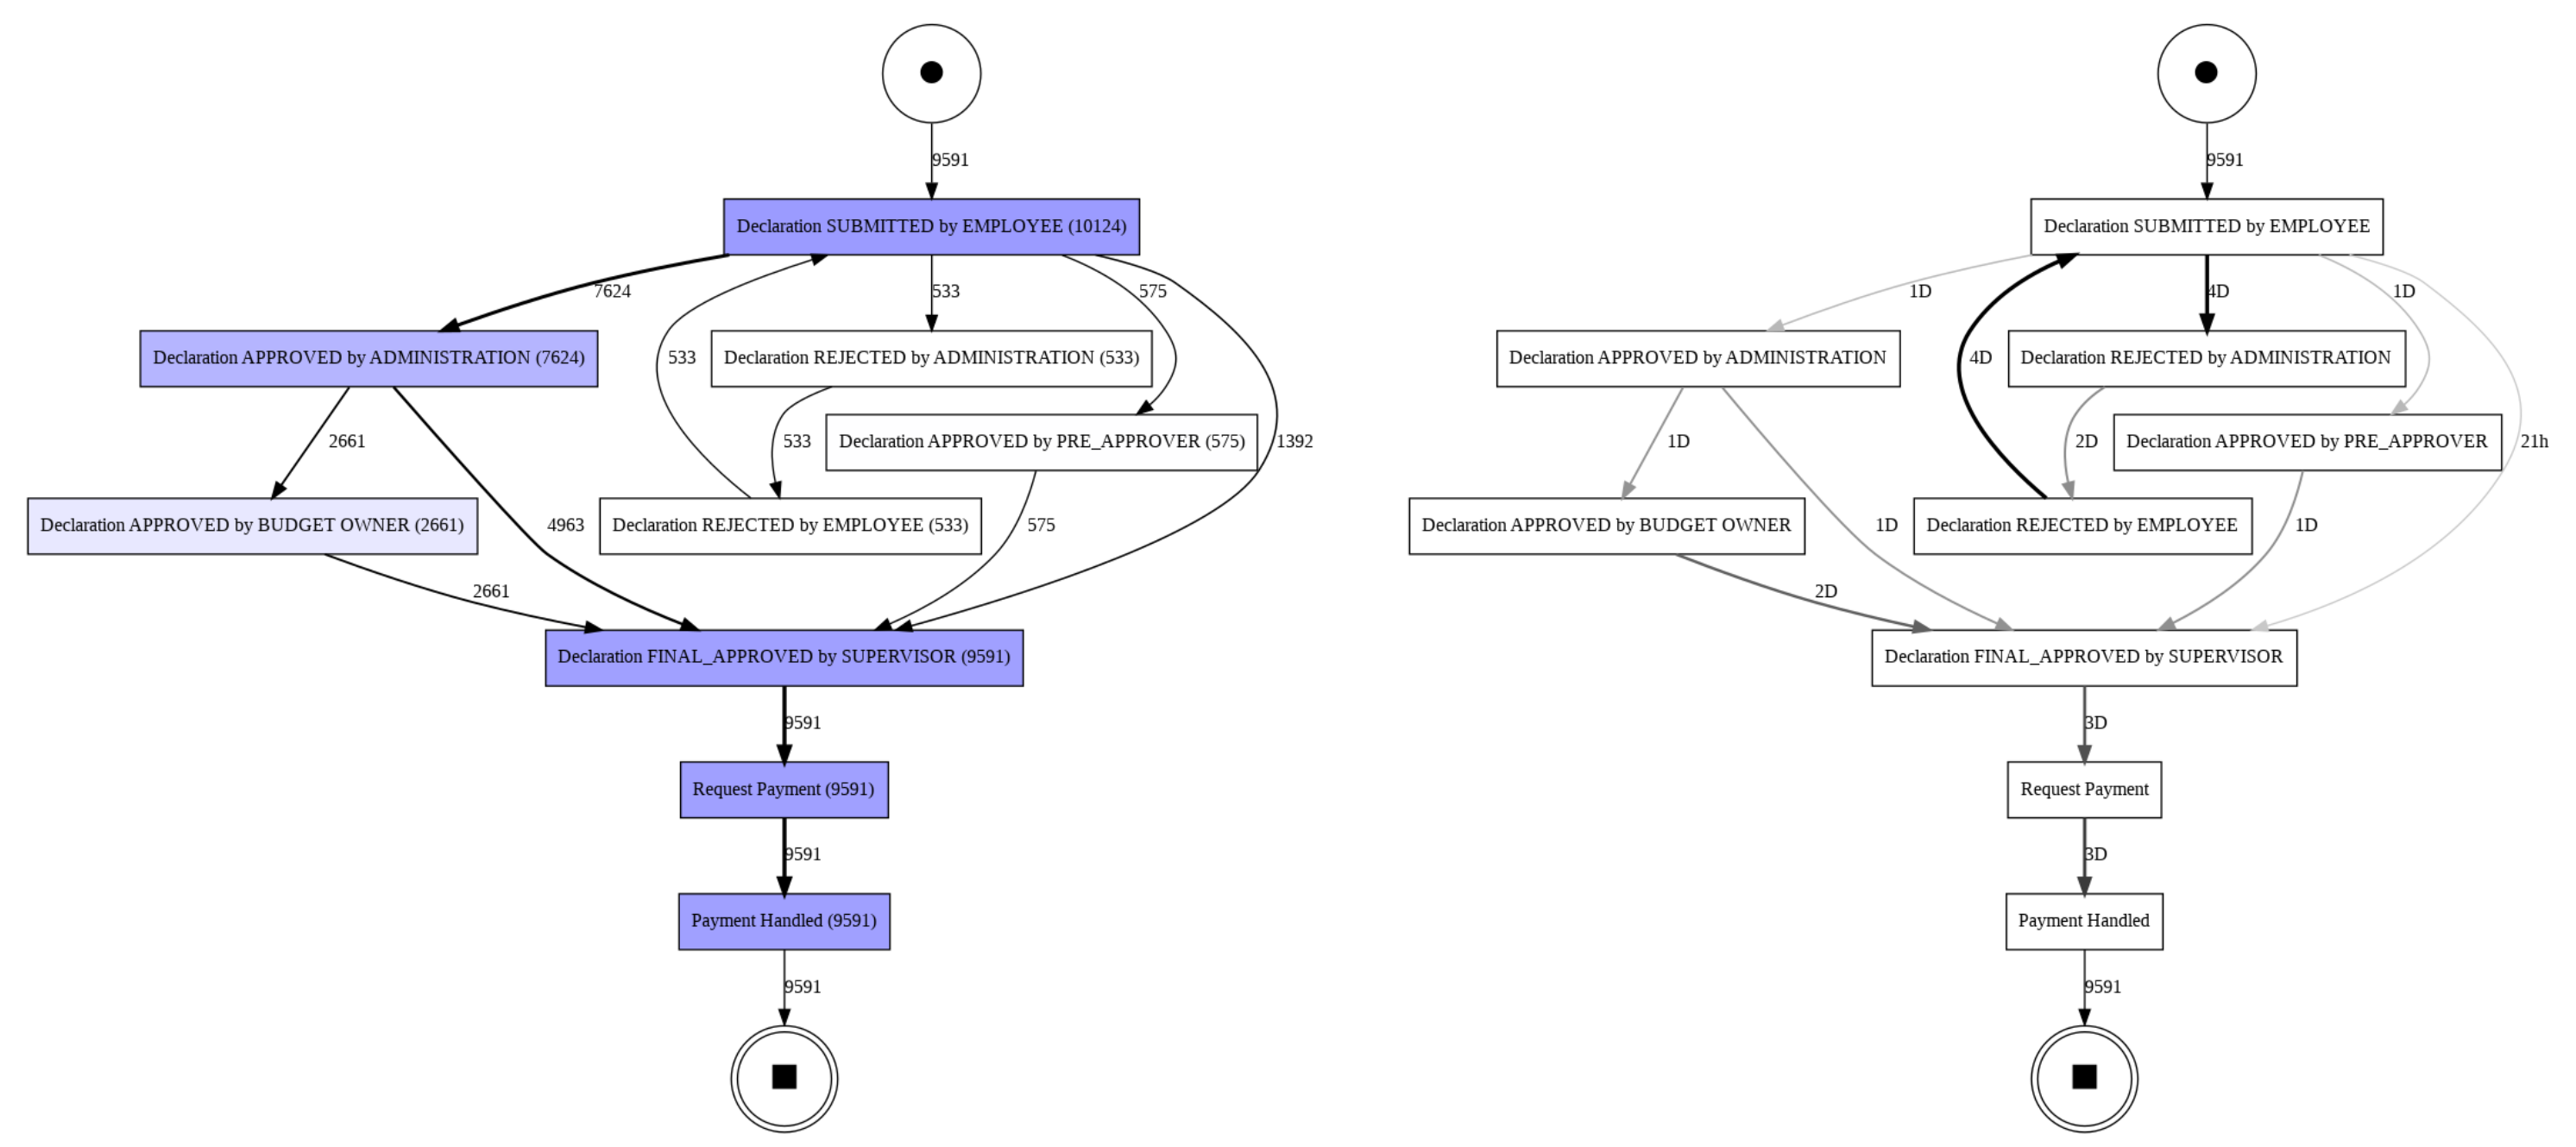
\includegraphics[width=0.90\textwidth]{images/domestic.png}}
\caption{DFG Model for Domestic Reimbursement.}
\label{fig-domestic}
\end{figure*}

\begin{figure*}[htbp]
\centerline{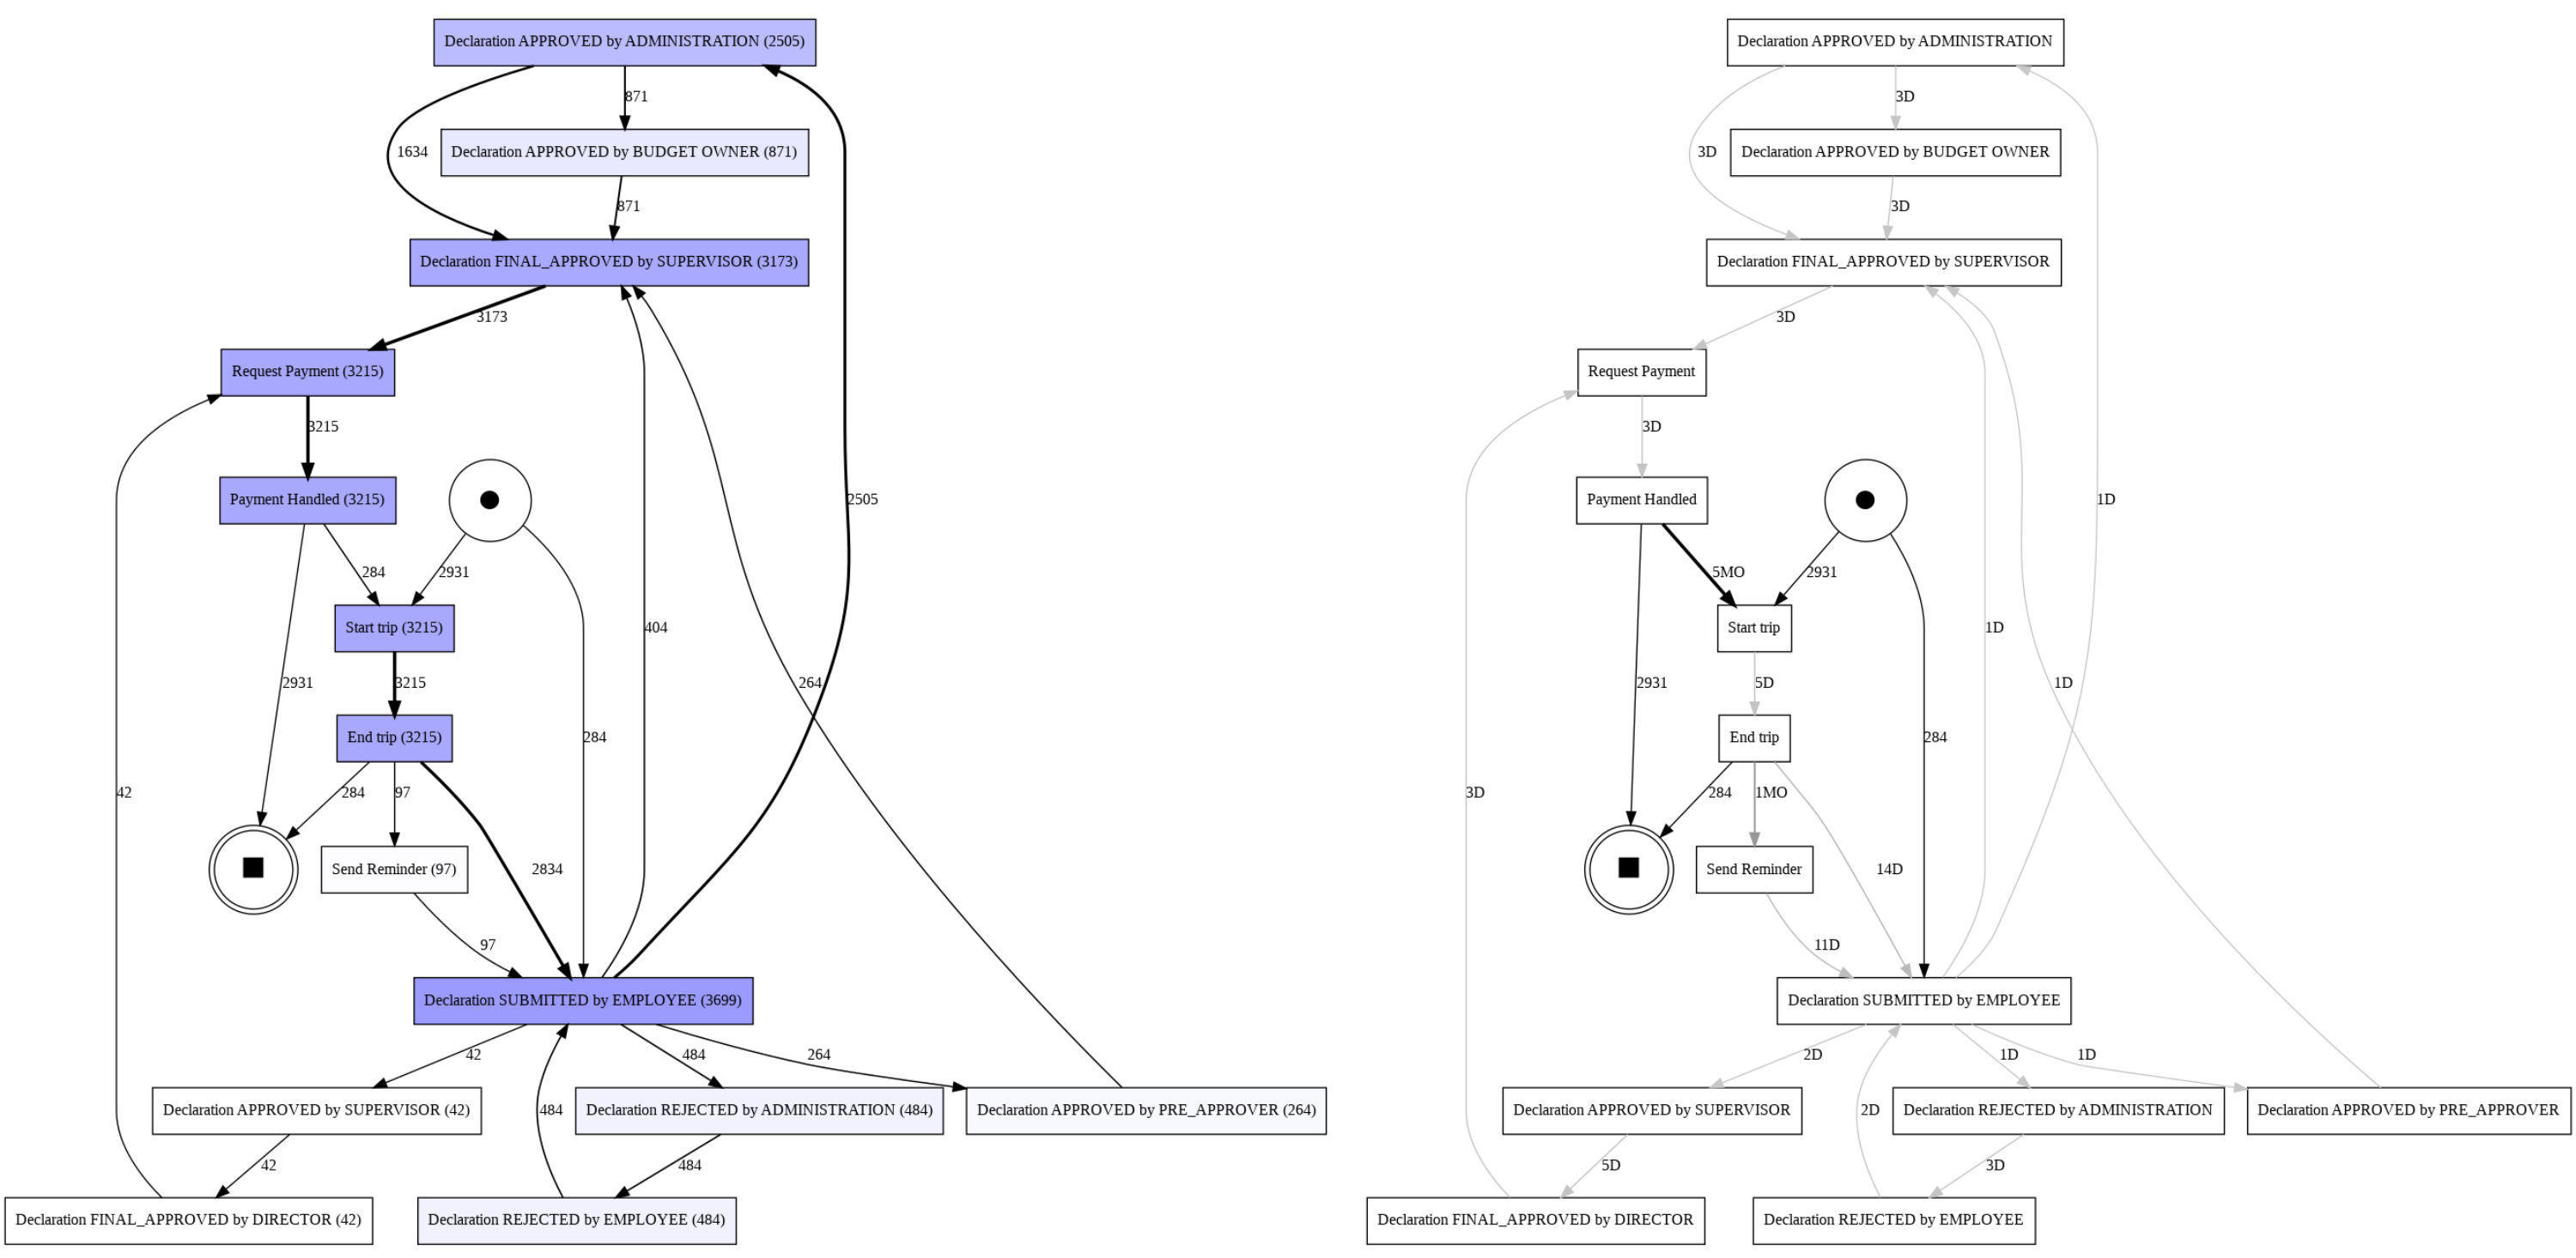
\includegraphics[width=0.90\textwidth]{images/international.png}}
\caption{DFG Model for International Reimbursement.}
\label{fig-international}
\end{figure*}


\subsection{Results}

Now that we have a robust process model built on reasonably clean data,
we can now answer the question: 
Where are the bottlenecks in the process of a travel declaration?

The biggest bottleneck is the supervisor activities for both International
and Domestic declarations. For the supervisor to do the final approval and
request payment, it takes an average of 4 to 5 days.
If we simply have to identify one activity, \textsc{Payment Handled}
is the biggest bottleneck. That said,
it might be outside of the organization’s control and may be more of a
financial institution issue.

Note that \textsc{pm4py} does not allow us to customize the performance
graph output,
instead, it rounds up the time to days instead of leaving it in an hour format. Also, \textsc{pm4py} does not have a method of superimposing the frequency and performance.


\section{Future Work}
\label{section-future}

\subsection{Conformance Analysis}

Once we have developed a process model either extracted through process
discovery, or built on some reference guidelines. It would be
interesting to investigate further into conformance checking to see how
well the data fits the model, while in turn would help us evaluate and
improve on the model.

This can be done with a method called token-based replay (TBR) on the
Petri-net converted from the process model. For each trace, we would try
to see if it can be executed on the petri-net in a mathematically sound
way, keeping track of additional tokens added to avoid deadlock, and
check for unused tokens at completion. We define the total fitness
simply as the percentage of traces that fit the model. Another technique
is alignment analysis, which is similar to TBR, except that events of a
trace are aligned to a legal and model-fitting trace trajectory subject
to certain cost functions. TBR and alignment analysis would both
identify non-conformance, but the latter is more informative, although
it comes at the expense of runtime complexity. Behavior analysis entails
the analysis of concepts that are present in the event log but either
impossible or expensive to capture in the event formalism (e.g.~the
person who submits the request cannot be the same person who approves).
These techniques can be used to better identify the hows and whys of
non-conformance, and to build better models.

Getting to 100\% total fitness is not necessarily a desired goal.
Instead, what we seek is a tradeoff. On the one hand, you want the model
to be robust enough to elegantly explain the process. On the other hand,
we do not want to over-build the model to make it so complex that it is
hard to reason about. Let's use our specific problem as an example. We
ran an experiment to examine such relationships. We ran the inductive
miner on different values of k, where k is the number of top variants we
used to build the model. And we ran the conformance check to get the
total fitness, and wrote code to examine the model. In this figure, the
red line is the total fitness, and the blue line is the size of the
model. We see that, as we include more traces, the model gets more
complex, but the fitness also improves. If we would include only the top
3 variants, we can explain 90\% of the traces. But if we blindly up the
ante to 18 variants, we can now account for 99\% of the traces, but the
model is 5 times bigger, and much harder to understand.

\begin{figure}[htbp]
\centerline{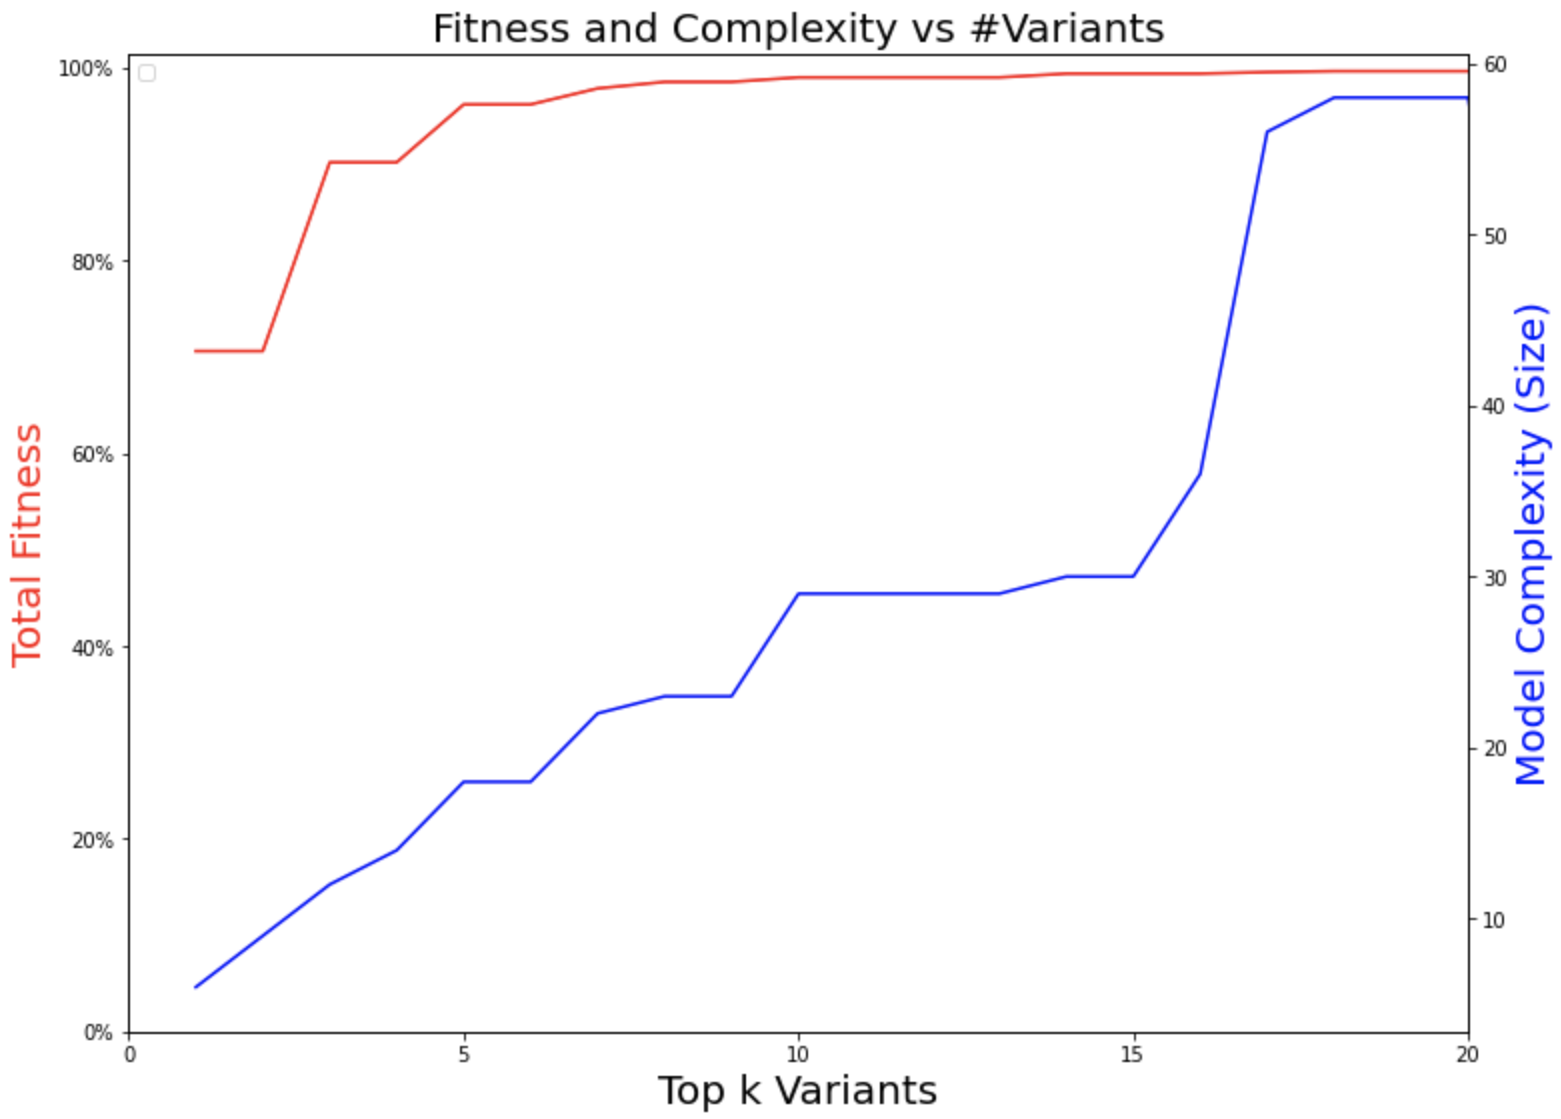
\includegraphics[width=0.45\textwidth]{images/tradeoff.png}}
\caption{Fitness and Complexity vs Top $k$ Variants.}
\label{fig}
\end{figure}

The sweat spots happen at k = 5, which can explain 96\% of the traces.
Moreover,
it can properly capture the submission, approval, rejection,
resubmission, and the final payment.

%\begin{figure}[htbp]
%\centerline{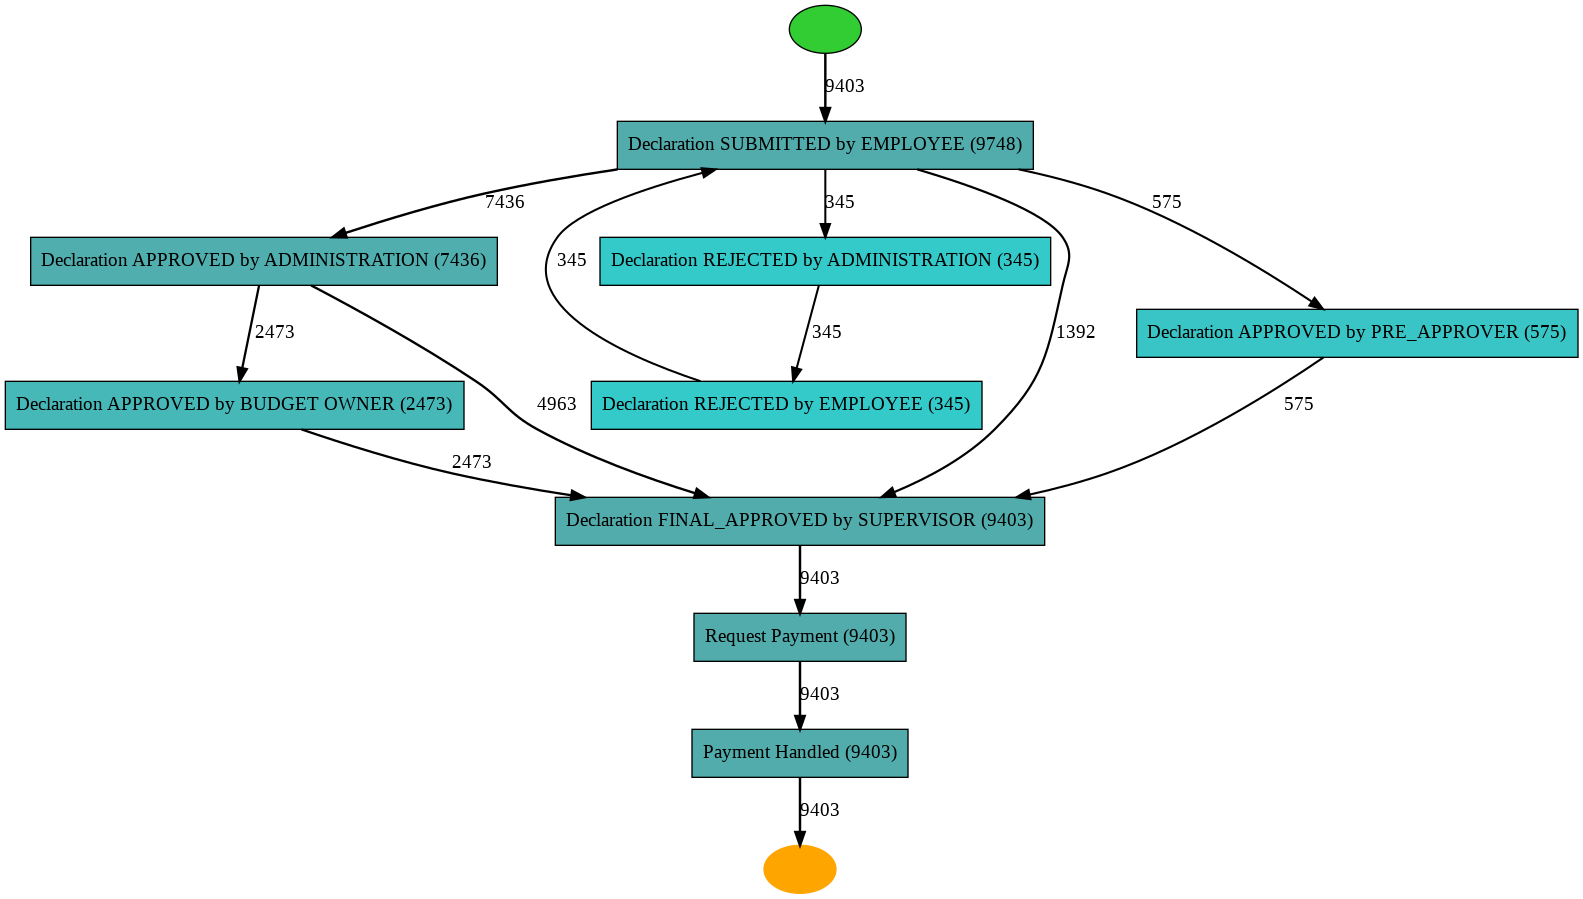
\includegraphics[width=0.45\textwidth]{images/heuristics_net_5.png}}
%\caption{Heuristics Net when using the Top 5 Variants.}
%\label{fig}
%\end{figure}

We have only scratched the surface of conformance analysis, as much more
can be done.

\subsection{Machine Learning and Timely
Analysis}

Another area of interest is to apply machine learning techniques to
perform (1) flow analysis to predict likelihood of resubmission,
rejection, payment delay, or over-budget based on other variables (time
since submission, request amount, prior owner approval), and (2) timing
analysis to determine mean-time-to-trace-completion. This provides
important clues to administrators and employees alike about the time
frame of payment in the best-case scenario. We are also interested in
detecting non-compliance ``as it happens'' and sending alerts to
administrators.

\section{Conclusion}
\label{section-conclusion}

\bibliographystyle{plain}
\bibliography{paper}{}

\begin{center}
\noindent\rule{0.5\columnwidth}{0.4pt}
\end{center}

\section{Contributions}

We would like to thank Professor Mahima Agumbe Suresh for her teaching,
encouragement, and devotion to helping us and other students succeed.
The following is a breakdown of our individual contributions:

\begin{itemize}
\item \textbf{Martin Alvarez-Lopez} -- advocated for the original proposal,
and set the overall direction of the project. He contributed to
data preparation, the main body of work on process mining, and gave the main
part of the presentation.

\item
\textbf{Carlos Hernandez} -- wrote the first draft of the term paper,
completed with extensive literature survey, project outline,
report template, as well as a significant portion of the writeup.

\item
\textbf{Hardy Leung} -- did an early investigation on \textsc{pm4py}, and
worked on conformance analysis. He also migrated the paper to the IEEE
template, and wrote the second half of the term paper.

\item
\textbf{Divyam Sobti} -- worked closely with Martin A.~on data preparation as
well as the main investigation on process mining. He set up the CoLab
environment, and contributed to report writing as well.

\end{itemize}

\end{document}
